\documentclass[draft=false,twoside,12pt]{scrreprt}
\newcommand{\lang}{english}
\usepackage[\lang]{babel}
\usepackage{graphicx}
\usepackage{float} %TODO what does this do
\usepackage[a4paper, 
            width = 150mm, top = 25mm, bottom = 25mm,
            bindingoffset = 6mm]
            {geometry}
% \usepackage{fancyhdr}
\usepackage{datatool}


\pagestyle{headings}

% \setlength{\parindent}{0pt}

% used packages

\usepackage[utf8]{inputenc}
\usepackage{graphicx}

% --- REFERENCING I-------------------------------------------------------------

\usepackage[hidelinks]{hyperref} % has to be loaded before ams to avoid warnings

%TODO
\usepackage[backend=biber, style = alphabetic]{biblatex}
\addbibresource{sourcesBergmannBT.bib}

% --- MATH ---------------------------------------------------------------------

\usepackage{amsmath} % align
\usepackage{amsthm} % proof
\usepackage{amssymb}
\usepackage{mathtools} %coloneqq
\usepackage{mathabx} %vvvert


% --- REFERENCING II -----------------------------------------------------------

\usepackage[\lang]{cleveref} % has to be loaded after ams and hyperref

% --- MISCELLANEOUS ------------------------------------------------------------

\usepackage{ifthen}


%\usepackage{tikz}
%\usepackage{pgfplots}
\usetikzlibrary{arrows.meta}

% --- AMSTHM ENVIRONMENtS ------------------------------------------------------

\theoremstyle{plain}
\newtheorem{theorem}{Theorem}[chapter]
\newtheorem{lemma}[theorem]{Lemma}
\newtheorem{corollary}[theorem]{Corollary}

\theoremstyle{definition}
\newtheorem{definition}[theorem]{Definition}

\theoremstyle{remark}
\newtheorem{remark}[theorem]{Remark}

% --- OPERATORS ----------------------------------------------------------------

\DeclareMathOperator{\interior}{int}
\DeclareMathOperator{\closure}{cl}
\DeclareMathOperator{\sign}{sign}
\DeclareMathOperator{\sgn}{sgn}
\DeclareMathOperator{\Div}{div}
\DeclareMathOperator{\atan}{atan2}
\DeclareMathOperator{\Curl}{Curl}
\newcommand{\conv}{\textup{conv}}
\newcommand{\Mid}{\textup{mid}}

%\DeclareMathOperator*{\liminf}{lim\,inf} % lim inf

% --- SPACES -------------------------------------------------------------------

\newcommand{\BV}{\textup{BV}}
\newcommand{\CR}{\textup{CR}}
\newcommand{\C}{\textup{C}}
\newcommand{\Vnc}{\ensuremath{V_\textup{NC}}}
% already defined\newcommand{\P}{\textup{P}}

% --- VARIABLES ----------------------------------------------------------------

\newcommand{\ucr}{u_\textup{CR}}
\newcommand{\vcr}{v_\textup{CR}}
\newcommand{\snr}{\textup{SNR}}
\newcommand{\Egleb}{E_\textup{GLEB}}

% --- FUNCTIONS ----------------------------------------------------------------

\newcommand{\Enc}{E_\textup{NC}}
\newcommand{\anc}{a_\textup{NC}}

% --- SYMBOLS/OPERATORS --------------------------------------------------------

\newcommand{\nc}{\textup{NC}}
\newcommand{\NC}{\textup{NC}}
\newcommand{\dx}{\,\mathrm{d}x}
\newcommand{\ds}{\,\mathrm{d}s}
\newcommand{\dt}{\,\mathrm{d}t}
\newcommand{\dmu}{\,\mathrm{d}\mu}
\newcommand{\gradnc}{\nabla_\textup{NC}}

% --- RELATIONS ----------------------------------------------------------------

\newcommand{\ssubset}{\subset\joinrel\subset}

% --- CALIGRAPHIC LETTERS ------------------------------------------------------

\newcommand\Acal{\mathcal{A}}
\newcommand\Bcal{\mathcal{B}}
\newcommand\Ccal{\mathcal{C}}
\newcommand\Dcal{\mathcal{D}}
\newcommand\Ecal{\mathcal{E}}
\newcommand\Fcal{\mathcal{F}}
\newcommand\Gcal{\mathcal{G}}
\newcommand\Hcal{\mathcal{H}}
\newcommand\Ical{\mathcal{I}}
\newcommand\Jcal{\mathcal{J}}
\newcommand\Kcal{\mathcal{K}}
\newcommand\Lcal{\mathcal{L}}
\newcommand\Mcal{\mathcal{M}}
\newcommand\Ncal{\mathcal{N}}
\newcommand\Ocal{\mathcal{O}}
\newcommand\Pcal{\mathcal{P}}
\newcommand\Qcal{\mathcal{Q}}
\newcommand\Rcal{\mathcal{R}}
\newcommand\Scal{\mathcal{S}}
\newcommand\Tcal{\mathcal{T}}
\newcommand\Ucal{\mathcal{U}}
\newcommand\Vcal{\mathcal{V}}
\newcommand\Wcal{\mathcal{W}}
\newcommand\Xcal{\mathcal{X}}
\newcommand\Ycal{\mathcal{Y}}
\newcommand\Zcal{\mathcal{Z}}

% --- MATHBB LETTERS -----------------------------------------------------------

\newcommand\Abb{\mathbb{A}}
%\newcommand\Bbb{\mathbb{B}}
\newcommand\Cbb{\mathbb{C}}
\newcommand\Dbb{\mathbb{D}}
\newcommand\Ebb{\mathbb{E}}
\newcommand\Fbb{\mathbb{F}}
\newcommand\Gbb{\mathbb{G}}
\newcommand\Hbb{\mathbb{H}}
\newcommand\Ibb{\mathbb{I}}
\newcommand\Jbb{\mathbb{J}}
\newcommand\Kbb{\mathbb{K}}
\newcommand\Lbb{\mathbb{L}}
\newcommand\Mbb{\mathbb{M}}
\newcommand\Nbb{\mathbb{N}}
\newcommand\Obb{\mathbb{O}}
\newcommand\Pbb{\mathbb{P}}
\newcommand\Qbb{\mathbb{Q}}
\newcommand\Rbb{\mathbb{R}}
\newcommand\Sbb{\mathbb{S}}
\newcommand\Tbb{\mathbb{T}}
\newcommand\Ubb{\mathbb{U}}
\newcommand\Vbb{\mathbb{V}}
\newcommand\Wbb{\mathbb{W}}
\newcommand\Xbb{\mathbb{X}}
\newcommand\Ybb{\mathbb{Y}}
\newcommand\Zbb{\mathbb{Z}}

% --- INTEGRAL MEAN ------------------------------------------------------------

\def\Xint#1{\mathchoice
{\XXint\displaystyle\textstyle{#1}}%
{\XXint\textstyle\scriptstyle{#1}}%
{\XXint\scriptstyle\scriptscriptstyle{#1}}%
{\XXint\scriptscriptstyle\scriptscriptstyle{#1}}%
\!\int}
\def\XXint#1#2#3{{\setbox0=\hbox{$#1{#2#3}{\int}$}
\vcenter{\hbox{$#2#3$}}\kern-.5\wd0}}
\newcommand{\intmean}{\Xint-}

% --- PERFECT BULLET -----------------------------------------------------------

\let\oldbullet\bullet
\newlength{\raisebulletlen}
\setbox1=\hbox{$\bullet$}\setbox2=\hbox{\tiny$\bullet$}
\setlength{\raisebulletlen}{\dimexpr0.5\ht1-0.5\ht2}
\renewcommand\bullet{\raisebox{\raisebulletlen}{\,\tiny$\oldbullet$}\,}
 

\begin{document}
\section{The continuous and discrete problem}
Let $\alpha>0$, $\Omega\subset\Rbb^n$ bounded polyhedral Lipschitz domain, and
$f\in L^2(\Omega)$.

The continuous problem minimizes 
\begin{align}
  \label{equ:contProb}
  E(v)\coloneqq \frac{\alpha}{2}\Vert v\Vert^2_{L^2(\Omega)}
  +|v|_{\BV(\Omega)}+ \Vert v\Vert_{L^1(\partial\Omega)}
  -\int_\Omega f\,v\dx
\end{align}
amongst all $v\in V\coloneqq \BV(\Omega)\cap L^2(\Omega)$ where the \BV 
seminorm $|v|_{\BV(\Omega)}$ is equal to the $W^{1,1}$ seminorm for any 
$v\in W^{1,1}(\Omega)$.

The nonconforming problem minimizes 
\begin{align}
  \label{equ:discProb}
  \Enc(\vcr)\coloneqq \frac{\alpha}{2}\Vert \vcr\Vert^2_{L^2(\Omega)}
  +|\vcr |_{1,1,\NC}-\int_\Omega f\, \vcr\dx
\end{align}
amongst all $\vcr\in\CR^1_0(\Tcal)$ where $|\bullet|_{1,1,\NC}\coloneqq
\Vert\gradnc\bullet\Vert_{L^1(\Omega)}$.

\section{Refinement indicator and guaranteed lower energy bound}

For some $n\in\mathbb{N}$ (here $n=2$) and $0<\gamma\leq 1$ define a refinement
indicator 
$\eta\coloneqq\sum_{T\in\mathcal{T}}\eta(T)$
with
\begin{align}
  \label{equ:errorEstimator}
  \eta (T)\coloneqq 
  \underbrace{|T|^{2/n}\Vert f-\alpha \ucr\Vert^2_{L^2(T)}}_{\eqqcolon 
  \eta_\text{Vol}(T)}
  +\underbrace{|T|^{\gamma/n}\sum_{F\in\Fcal(T)}\Vert [\ucr]_F\Vert_{L^1(F)}}_{
  \eqqcolon \eta_\text{Jumps}(T)}
\end{align}
for any $T\in\mathcal{T}$.

For $f\in H^1_0(\Omega)$ and $u\in H^1_0(\Omega)$ $\left(\ucr\in
\CR^1_0(\Omega)\right)$ continuous (discrete) minimizer with minimal energy
$E(u)$ $\left(\Enc(\ucr)\right)$ it holds
\begin{align}
  \label{equ:gleb}
  \Enc(\ucr)+\frac{\alpha}{2}\Vert u-\ucr\Vert_{L^2(\Omega)}^2
  -\frac{\kappa_\CR}{\alpha}\Vert
  h_\mathcal{T}(f-\alpha\ucr)\Vert_{L^2(\Omega)} |f|_{1,2}\leq E(u)
\end{align}
where $|\bullet|_{1,2}=\Vert\nabla \bullet\Vert_{L^2(\Omega)}$.

Hence, for $\textup{GLEB} \coloneqq 
  \Enc(\ucr) - \frac{\kappa_\CR}{\alpha}\Vert
  h_\mathcal{T}(f-\alpha\ucr)\Vert_{L^2(\Omega)} |f|_{1,2}$, it holds
  $\Enc(\ucr)\geq \textup{GLEB}$ and $E(u)\geq \textup{GLEB}$.

\section{Experiments}
In the following sections on each level the termination criterion for the
iteration was
\begin{align*}
  \left\Vert \frac{\gradnc (u_{j}-u_{j-1})}{\tau}  \right\Vert_{L^2(\Omega)}
  <\varepsilon\coloneqq 10^{-4}
\end{align*}
for $\tau=\frac{1}{2}$.

\section{Examples with exact solution}
\subsection{Example 1}
For $\beta=1$ define $f$ as a function of the radius as
\begin{align}
  \label{equ:f01}
  f(r)\coloneqq 
  \begin{cases}
    \alpha-12(2-9r) & \text{if } 0\leq r\leq\frac{1}{6},\\
    \alpha(1+(6r-1)^\beta)-\frac{1}{r} & \text{if } \frac{1}{6}\leq r\leq
    \frac{1}{3},\\
    2\alpha+6\pi\sin(\pi(6r-2))-\frac{1}{r}\cos(\pi(6r-2)) &
    \text{if } \frac{1}{3}\leq r\leq\frac{1}{2},\\
    2\alpha(\frac{5}{2}-3r)^\beta+\frac{1}{r}&
    \text{if } \frac{1}{2}\leq r\leq\frac{5}{6},\\
    -3\pi\sin(\pi(6r-5))+\frac{1+\cos(\pi(6r-5))}{2r} &
    \text{if } \frac{5}{6}\leq r\leq 1,
  \end{cases}
\end{align}
with exact solution
\begin{align}
  \label{equ:f01exactSol}
  u(r)\coloneqq
  \begin{cases}
    1 & \text{if } 0\leq r\leq\frac{1}{6},\\
    1+(6r-1)^\beta & \text{if } \frac{1}{6}\leq r\leq
    \frac{1}{3},\\
    2 &
    \text{if } \frac{1}{3}\leq r\leq\frac{1}{2},\\
    2(\frac{5}{2}-3r)^\beta &
    \text{if } \frac{1}{2}\leq r\leq\frac{5}{6},\\
    0 &
    \text{if } \frac{5}{6}\leq r\leq 1.
  \end{cases}
\end{align}

For $\alpha=1$ the exact energy $E(u)$ was computed before the experiment.

\begin{minipage}[t]{0.3\textwidth}
  \begin{figure}[H]
	  \centering
		\includegraphics[width=1.1\textwidth]{tikzPlots/f01/alpha1/rhs.png} 
		\caption{$f$ for $\alpha=1$}
  \end{figure}
\end{minipage}
\hfill
\vline
\hfill
\begin{minipage}[t]{0.3\textwidth}
  \begin{figure}[H]
	  \centering
		\includegraphics[width=1.1\textwidth]{tikzPlots/f01/alpha1e4/rhs.png} 
		\caption{$f$ for $\alpha=10^4$}
  \end{figure}
\end{minipage}
\hfill
\vline
\hfill
\begin{minipage}[t]{0.3\textwidth}
  \begin{figure}[H]
	  \centering
		\includegraphics[width=1.1\textwidth]
    {tikzPlots/f01/alpha1/exactSolution.png} 
		\caption{$u$}
  \end{figure}
\end{minipage}

\begin{minipage}[t]{0.3\textwidth}
  \begin{figure}[H]
	  \centering
		\includegraphics[width=1.1\textwidth]{tikzPlots/f01/alpha1/rhsAxis.png} 
		\caption{$f$ along the axes for $\alpha=1$}
  \end{figure}
\end{minipage}
\hfill
\vline
\hfill
\begin{minipage}[t]{0.3\textwidth}
  \begin{figure}[H]
	  \centering
		\includegraphics[width=1.1\textwidth]{tikzPlots/f01/alpha1e4/rhsAxis.png} 
		\caption{$f$ along the axes for $\alpha=10^4$}
  \end{figure}
\end{minipage}
\hfill
\vline
\hfill
\begin{minipage}[t]{0.3\textwidth}
  \begin{figure}[H]
	  \centering
		\includegraphics[width=1.1\textwidth]
    {tikzPlots/f01/alpha1/exactSolutionAxis.png} 
		\caption{$u$ along the axes}
  \end{figure}
\end{minipage}

\vspace{-\parskip}
\begin{figure}[H]
	\centering
	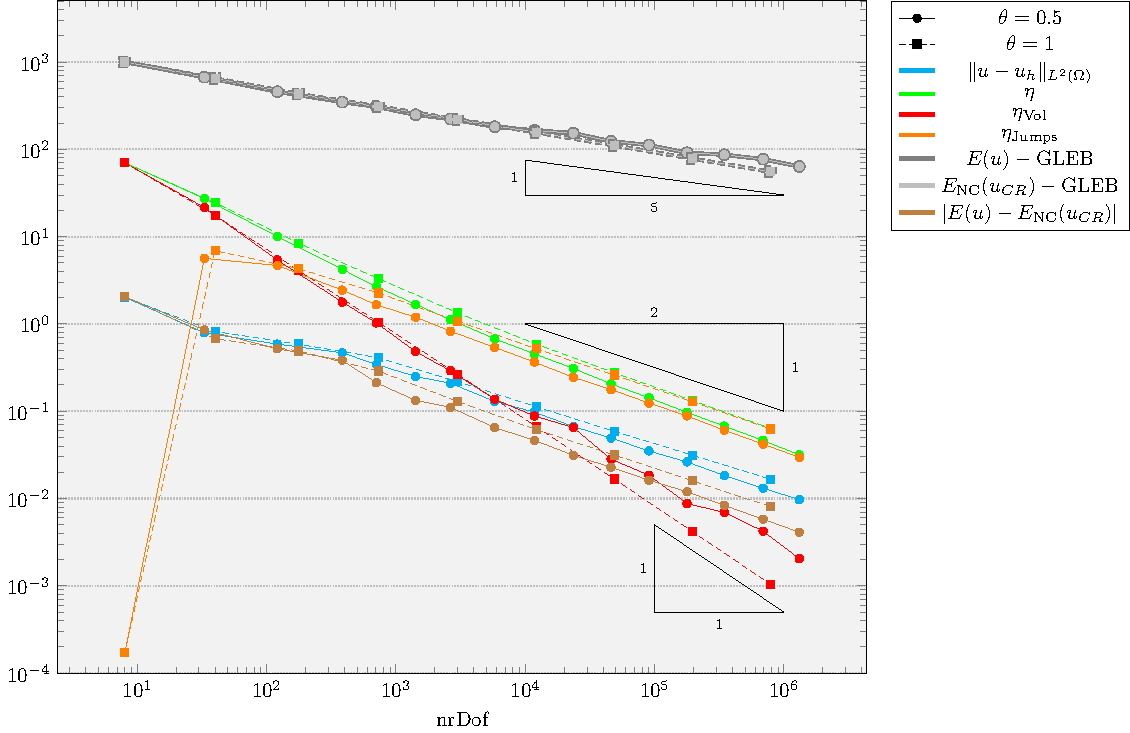
\includegraphics[width=14cm]{tikzPlots/f01/alpha1/convergence.pdf}
  \caption{convergence history plot for $\alpha=1$}
\end{figure}

\vspace{-\parskip}
\begin{figure}[H]
	\centering
	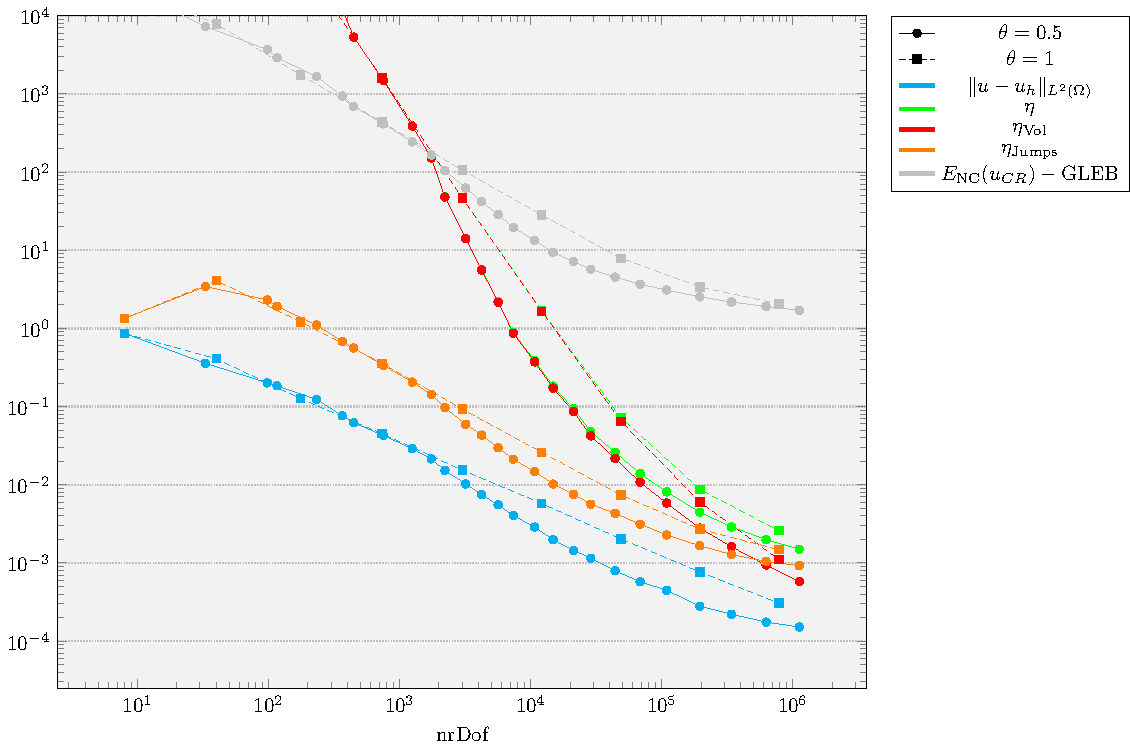
\includegraphics[width=14cm]{tikzPlots/f01/alpha1e4/convergence.pdf}
  \caption{convergence history plot for $\alpha=10^4$}
\end{figure}

\vspace{-\parskip}
\begin{figure}[H]
	\centering
	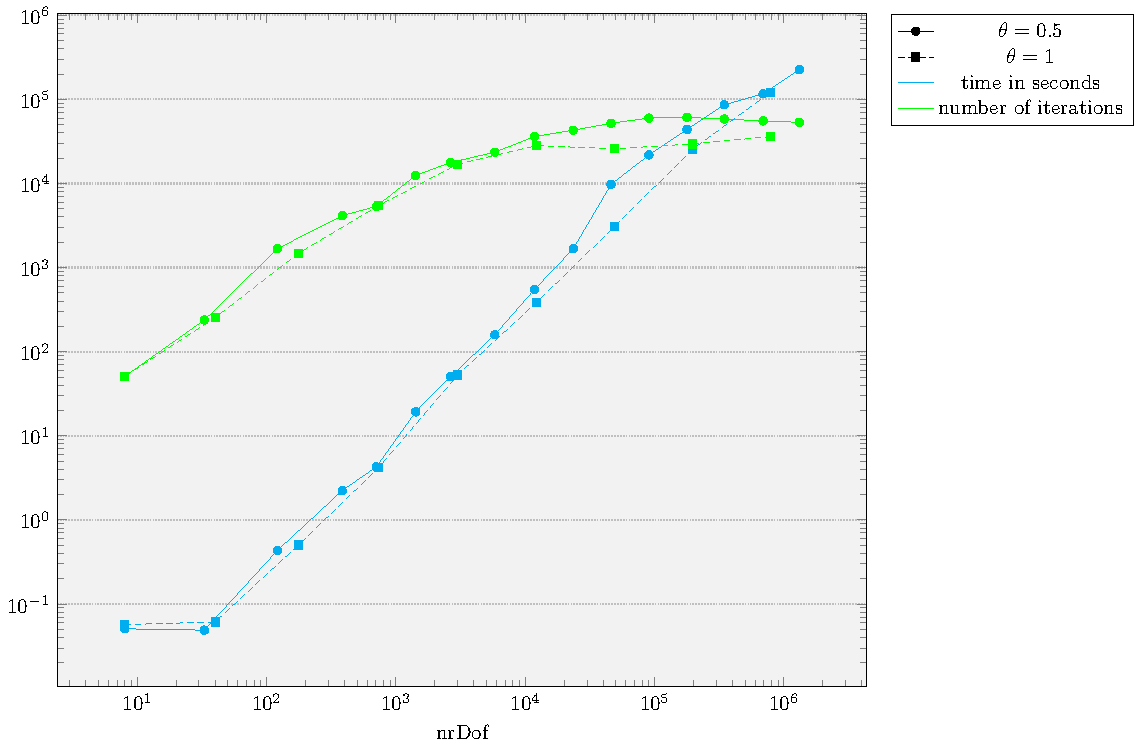
\includegraphics[width=14cm]{tikzPlots/f01/alpha1/misc.pdf}
  \caption{development of the number of iterations and the elapsed time for 
  each iteration for $\alpha=1$}
\end{figure}

\vspace{-\parskip}
\begin{figure}[H]
	\centering
	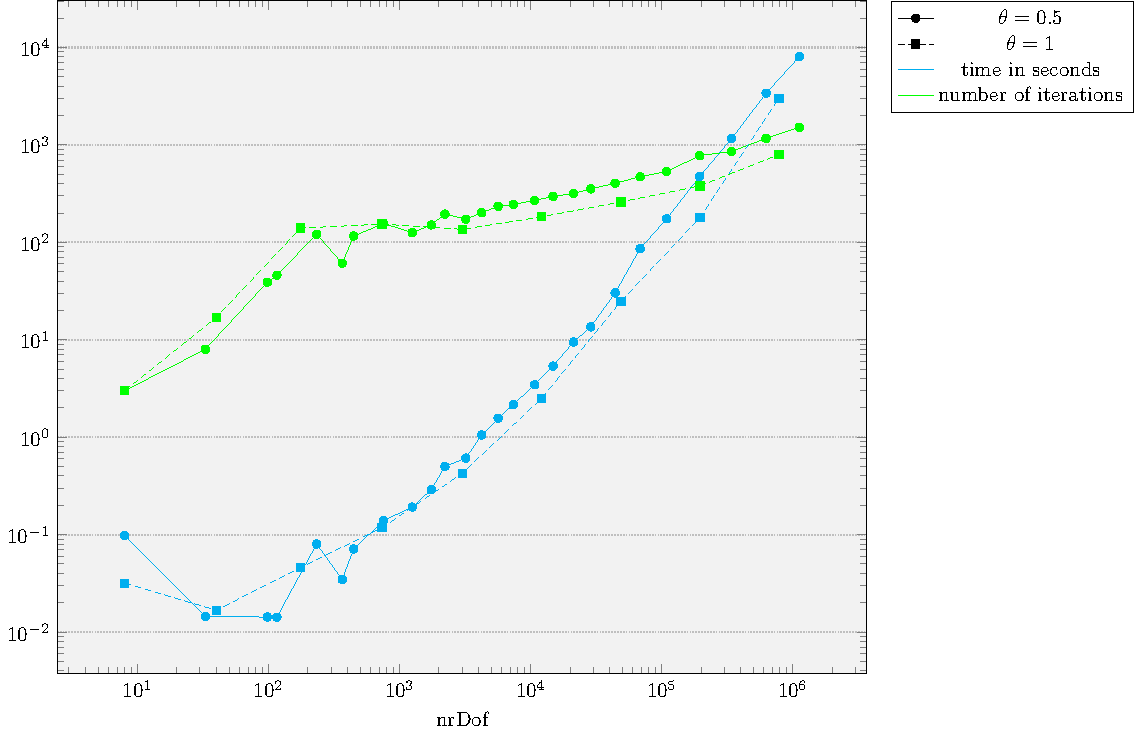
\includegraphics[width=14cm]{tikzPlots/f01/alpha1e4/misc.pdf}
  \caption{development of the number of iterations and the elapsed time for 
  each iteration for $\alpha=10^4$}
\end{figure}

\DTLloaddb{db}{tikzPlots/f01/alpha1/1e-4/adaptive/lvl10/currentDataReduced.csv}
\DTLassign{db}{1}{\nrNodes=nrNodes, \nrDof=nrDof}

\DTLloaddb{dbAlt}{tikzPlots/f01/alpha1e4/1e-4/adaptive/lvl19/currentDataReduced.csv}
\DTLassign{dbAlt}{1}{\nrNodesAlt=nrNodes, \nrDofAlt=nrDof}

\vspace{-\parskip}
\begin{minipage}[t]{0.45\textwidth}
  \begin{figure}[H]
    \includegraphics[width=1.3\textwidth]
    {tikzPlots/f01/alpha1/1e-4/adaptive/lvl10/triangulation.png}
    \caption{adaptive mesh for $\alpha=1$ and $\theta = 0.5$ with \nrNodes\
    nodes and \nrDof\ degrees of freedom}
  \end{figure}
\end{minipage}
\hfill
\vline
\hfill
\begin{minipage}[t]{0.45\textwidth}
  \begin{figure}[H]
  	\centering
    \includegraphics[width=1.3\textwidth]
    {tikzPlots/f01/alpha1e4/1e-4/adaptive/lvl19/triangulation.png}
    \caption{adaptive mesh for $\alpha=10^4$ and $\theta = 0.5$ with
    \nrNodesAlt\ nodes and \nrDofAlt\ degrees of freedom}
  \end{figure}
\end{minipage}

\DTLgdeletedb{db}
\DTLgdeletedb{dbAlt}

\begin{minipage}[t]{0.45\textwidth}
  \begin{figure}[H]
	  \centering
		\includegraphics[width=1.1\textwidth]
      {tikzPlots/f01/alpha1/1e-4/adaptive/lvl15/solution.png} 
    \caption{last iterate for $\alpha=1$ and $\theta = 0.5$}
  \end{figure}
\end{minipage}
\hfill
\vline
\hfill
\begin{minipage}[t]{0.45\textwidth}
  \begin{figure}[H]
	  \centering
		\includegraphics[width=1.1\textwidth]
      {tikzPlots/f01/alpha1/1e-4/uniform/lvl8/solution.png} 
    \caption{last iterate for $\alpha=1$ and $\theta = 1$}
  \end{figure}
\end{minipage}

\vspace{-\parskip}
\begin{minipage}[t]{0.45\textwidth}
  \begin{figure}[H]
	  \centering
		\includegraphics[width=1.1\textwidth]
      {tikzPlots/f01/alpha1/1e-4/adaptive/lvl15/solutionAxis.png} 
    \caption{last iterate along the axes for $\alpha=1$ and $\theta = 0.5$}
  \end{figure}
\end{minipage}
\hfill
\vline
\hfill
\begin{minipage}[t]{0.45\textwidth}
  \begin{figure}[H]
	  \centering
		\includegraphics[width=1.1\textwidth]
      {tikzPlots/f01/alpha1/1e-4/uniform/lvl8/solutionAxis.png} 
    \caption{last iterate along the axes for $\alpha=1$ and $\theta = 1$}
  \end{figure}
\end{minipage}

\begin{minipage}[t]{0.45\textwidth}
  \begin{figure}[H]
	  \centering
		\includegraphics[width=1.1\textwidth]
      {tikzPlots/f01/alpha1e4/1e-4/adaptive/lvl25/solution.png} 
    \caption{last iterate for $\alpha=10^4$ and $\theta = 0.5$}
  \end{figure}
\end{minipage}
\hfill
\vline
\hfill
\begin{minipage}[t]{0.45\textwidth}
  \begin{figure}[H]
	  \centering
		\includegraphics[width=1.1\textwidth]
      {tikzPlots/f01/alpha1e4/1e-4/uniform/lvl8/solution.png} 
    \caption{last iterate for $\alpha=10^4$ and $\theta = 1$}
  \end{figure}
\end{minipage}

\vspace{-\parskip}
\begin{minipage}[t]{0.45\textwidth}
  \begin{figure}[H]
	  \centering
		\includegraphics[width=1.1\textwidth]
      {tikzPlots/f01/alpha1e4/1e-4/adaptive/lvl25/solutionAxis.png} 
    \caption{last iterate along the axes for $\alpha=10^4$ and $\theta = 0.5$}
  \end{figure}
\end{minipage}
\hfill
\vline
\hfill
\begin{minipage}[t]{0.45\textwidth}
  \begin{figure}[H]
	  \centering
		\includegraphics[width=1.1\textwidth]
      {tikzPlots/f01/alpha1e4/1e-4/uniform/lvl8/solutionAxis.png} 
    \caption{last iterate along the axes for $\alpha=10^4$ and $\theta = 1$}
  \end{figure}
\end{minipage}

\subsection{Example 2}
For $\alpha=1$ and $\beta\in(0,1)$ define $f$ as a function of the radius as
\begin{align*}
  f(r)\coloneqq 
  \begin{cases}
    \alpha - \frac{4}{1-\beta}\left(\frac{3}{1-\beta}r - 2\right) &
    \text{if } 0\leq r\leq\frac{1-\beta}{2},\\
    -\frac{\alpha}{\beta}\left( r-\frac{1+\beta}{2} \right) +\frac{1}{r} & 
    \text{if } \frac{1-\beta}{2}\leq r\leq \frac{1+\beta}{2},\\
    \frac{-4}{(\beta-1)^3}
    \left( 16r^2 -9(\beta+3)r + 12(\beta+1) - \frac{3\beta+1}{r}\right) & 
    \text{if } \frac{1+\beta}{2}\leq r\leq 1,
  \end{cases}
\end{align*}
with exact solution
\begin{align*}
  u_2(r)\coloneqq 
  \begin{cases}
    1 & \text{if } 0\leq r\leq\frac{1-\beta}{2},\\
    -\frac{1}{\beta}r + \frac{1+\beta}{2\beta} & 
    \text{if } \frac{1-\beta}{2}\leq r\leq \frac{1+\beta}{2},\\
    0 & \text{if } \frac{1+\beta}{2}\leq r.
  \end{cases}
\end{align*}

The experiments were conducted for $\beta = \frac{1}{10}, \frac{1}{2},
\frac{9}{10}$ and the corresponding exact energies were computed beforehand.

\vspace{-\parskip}
\begin{minipage}[t]{0.3\textwidth}
  \begin{figure}[H]
	  \centering
		\includegraphics[width=1.1\textwidth]{tikzPlots/f02/beta1Tenth/rhs.png} 
    \caption{$f$ for $\beta=\frac{1}{10}$}
  \end{figure}
\end{minipage}
\hfill
\vline
\hfill
\begin{minipage}[t]{0.3\textwidth}
  \begin{figure}[H]
	  \centering
		\includegraphics[width=1.1\textwidth]{tikzPlots/f02/beta5Tenth/rhs.png} 
    \caption{$f$ for $\beta=\frac{1}{2}$}
  \end{figure}
\end{minipage}
\hfill
\vline
\hfill
\begin{minipage}[t]{0.3\textwidth}
  \begin{figure}[H]
	  \centering
		\includegraphics[width=1.1\textwidth]{tikzPlots/f02/beta9Tenth/rhs.png} 
    \caption{$f$ for $\beta=\frac{9}{10}$}
  \end{figure}
\end{minipage}

\vspace{-\parskip}
\begin{minipage}[t]{0.3\textwidth}
  \begin{figure}[H]
	  \centering
		\includegraphics[width=1.1\textwidth]{tikzPlots/f02/beta1Tenth/rhsAxis.png} 
    \caption{$f$ along the axes for $\beta=\frac{1}{10}$}
  \end{figure}
\end{minipage}
\hfill
\vline
\hfill
\begin{minipage}[t]{0.3\textwidth}
  \begin{figure}[H]
	  \centering
		\includegraphics[width=1.1\textwidth]{tikzPlots/f02/beta5Tenth/rhsAxis.png} 
    \caption{$f$ along the axes for $\beta=\frac{1}{2}$}
  \end{figure}
\end{minipage}
\hfill
\vline
\hfill
\begin{minipage}[t]{0.3\textwidth}
  \begin{figure}[H]
	  \centering
		\includegraphics[width=1.1\textwidth]{tikzPlots/f02/beta9Tenth/rhsAxis.png} 
    \caption{$f$ along the axes for $\beta=\frac{9}{10}$}
  \end{figure}
\end{minipage}

\vspace{-\parskip}
\begin{minipage}[t]{0.3\textwidth}
  \begin{figure}[H]
	  \centering
    \includegraphics[width=1.1\textwidth]
    {tikzPlots/f02/beta1Tenth/exactSolution.png} 
    \caption{$u$ for $\beta=\frac{1}{10}$}
  \end{figure}
\end{minipage}
\hfill
\vline
\hfill
\begin{minipage}[t]{0.3\textwidth}
  \begin{figure}[H]
	  \centering
    \includegraphics[width=1.1\textwidth]
    {tikzPlots/f02/beta5Tenth/exactSolution.png} 
    \caption{$u$ for $\beta=\frac{1}{2}$}
  \end{figure}
\end{minipage}
\hfill
\vline
\hfill
\begin{minipage}[t]{0.3\textwidth}
  \begin{figure}[H]
	  \centering
    \includegraphics[width=1.1\textwidth]
    {tikzPlots/f02/beta9Tenth/exactSolution.png} 
    \caption{$u$ for $\beta=\frac{9}{10}$}
  \end{figure}
\end{minipage}

\vspace{-\parskip}
\begin{minipage}[t]{0.3\textwidth}
  \begin{figure}[H]
	  \centering
		\includegraphics[width=1.1\textwidth]
    {tikzPlots/f02/beta1Tenth/exactSolutionAxis.png} 
    \caption{$u$ along the axes for $\beta=\frac{1}{10}$}
  \end{figure}
\end{minipage}
\hfill
\vline
\hfill
\begin{minipage}[t]{0.3\textwidth}
  \begin{figure}[H]
	  \centering
		\includegraphics[width=1.1\textwidth]
    {tikzPlots/f02/beta5Tenth/exactSolutionAxis.png} 
    \caption{$u$ along the axes for $\beta=\frac{1}{2}$}
  \end{figure}
\end{minipage}
\hfill
\vline
\hfill
\begin{minipage}[t]{0.3\textwidth}
  \begin{figure}[H]
	  \centering
		\includegraphics[width=1.1\textwidth]
    {tikzPlots/f02/beta9Tenth/exactSolutionAxis.png} 
    \caption{$u$ along the axes for $\beta=\frac{9}{10}$}
  \end{figure}
\end{minipage}

\section{Application to image}
For $\alpha = 10000$ let $f$ represent the grayscale of an image in
$[0,1]^{256\times 256}$ multiplied with $\alpha$ scaled to the domain
$\Omega\in(0,1)^2$ as seen in \cref{fig:rhsCameraman}.

\begin{figure}[H]
	\centering
	\includegraphics[width=14cm]{tikzPlots/imageCameraman/rhsGrayscale.png}
  \caption{grayscale plot of the right-hand side $f$ (view from above onto the
  $x$-$y$ plane)}
  \label{fig:rhsCameraman}
\end{figure}

\begin{figure}[H]
	\centering
	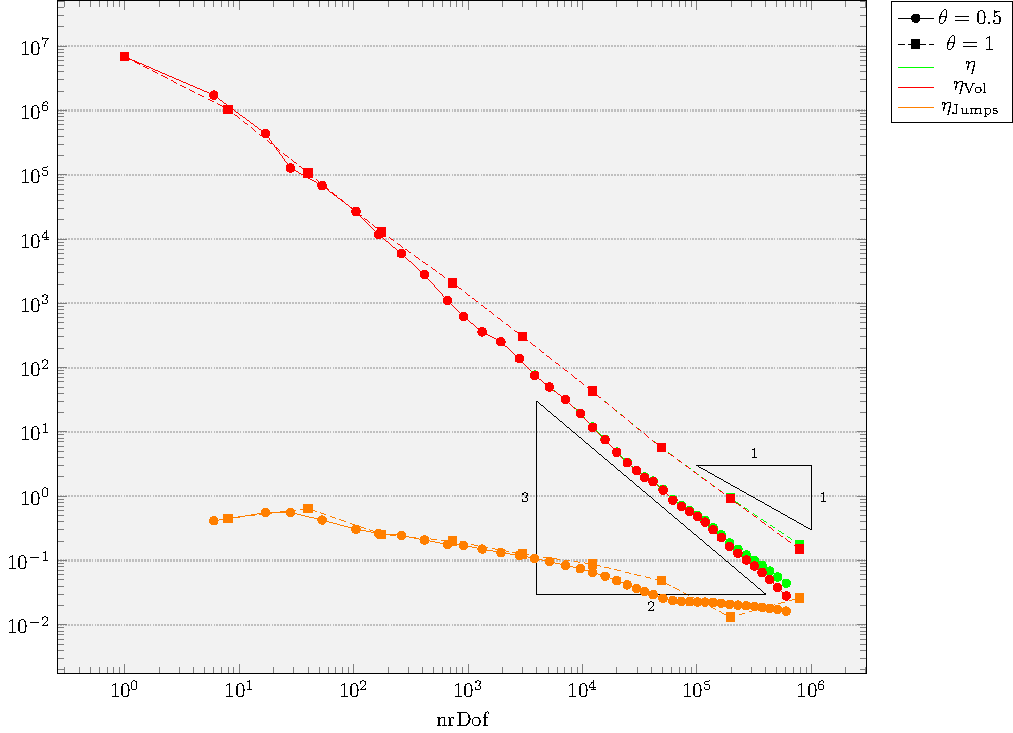
\includegraphics[width=14cm]
  {tikzPlots/imageCameraman/convergence.pdf}
  \caption{convergence history plot for $\eta$,
  $\eta_\text{Vol}$, and $\eta_\text{Jumps}$}
\end{figure}

\begin{figure}[H]
	\centering
	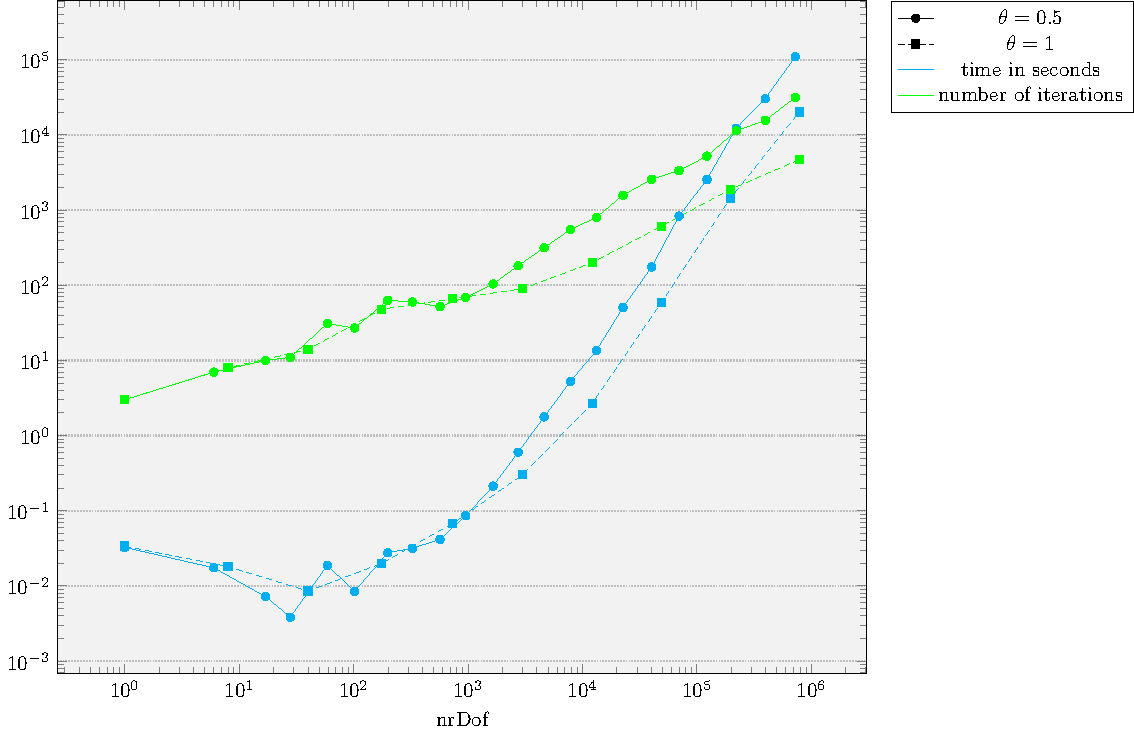
\includegraphics[width=14cm]{tikzPlots/imageCameraman/misc.pdf}
  \caption{development of the number of iterations and the elapsed time for 
  each iteration}
\end{figure}

\begin{minipage}[t]{0.5\textwidth}
  \begin{figure}[H]
	  \centering
		\includegraphics[width=\textwidth]
      {tikzPlots/imageCameraman/1e-4/adaptive/lvl21/solutionGrayscale.png}
    \caption{grayscale plot of last iterate for $\theta = 0.5$}
  \end{figure}
\end{minipage}
\begin{minipage}[t]{0.5\textwidth}
  \begin{figure}[H]
	  \centering
		\includegraphics[width=\linewidth]
      {tikzPlots/imageCameraman/1e-4/uniform/lvl9/solutionGrayscale.png}
    \caption{grayscale plot of last iterate for $\theta = 1$}
  \end{figure}
\end{minipage}

\DTLloaddb{db}{
tikzPlots/imageCameraman/1e-4/adaptive/lvl16/currentDataReduced.csv}
\DTLassign{db}{1}{\nrNodes=nrNodes, \nrDof=nrDof}

\begin{figure}[H]
	\centering
  \includegraphics[width=14cm]
  {tikzPlots/imageCameraman/1e-4/adaptive/lvl16/triangulation.png}
  \caption{adaptive mesh for $\theta = 0.5$ with \nrNodes\ nodes and 
  \nrDof\ degrees of freedom}
\end{figure}

\DTLgdeletedb{db}

%TODO here and above not only plot the mesh but also the solution on this mesh
%(maybe with subfigure or maybe with minipages)

\section{Application to a function with discontinuity set}
For $\alpha = 100$ define 
\begin{align}
  \label{equ:defMidSqu}
  f(x)\coloneqq 
  \begin{cases}
    100 &\text{if } \Vert x\Vert_\infty\leq \frac{1}{2},\\
    0 &\text{else}
  \end{cases}
\end{align}
on $\Omega = (-1,1)^2$.

\begin{figure}[H]
	\centering
	\includegraphics[width=14cm]{tikzPlots/middleSquare/rhsGrayscale.png}
  \caption{grayscale plot of the right-hand side $f$ (view from above onto the
  $x$-$y$ plane)}
  \label{fig:rhsMiddleSquare}
\end{figure}

\begin{figure}[H]
	\centering
	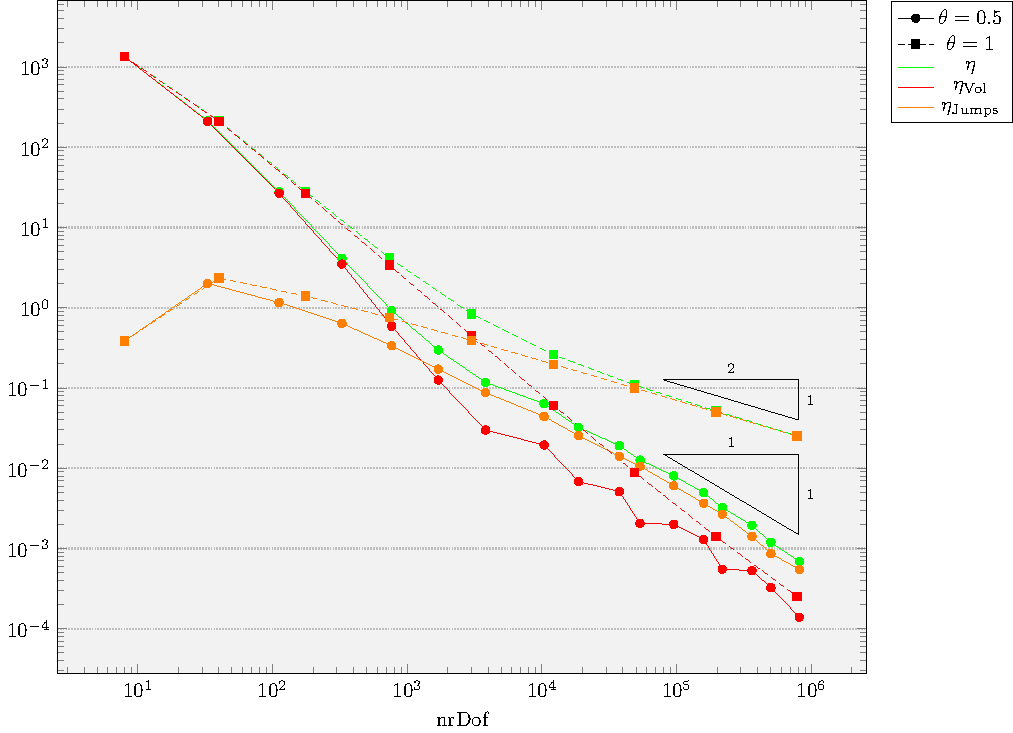
\includegraphics[width=14cm]
  {tikzPlots/middleSquare/convergence.pdf}
  \caption{convergence history plot for $\eta$,
  $\eta_\text{Vol}$, and $\eta_\text{Jumps}$}
\end{figure}

\begin{figure}[H]
	\centering
	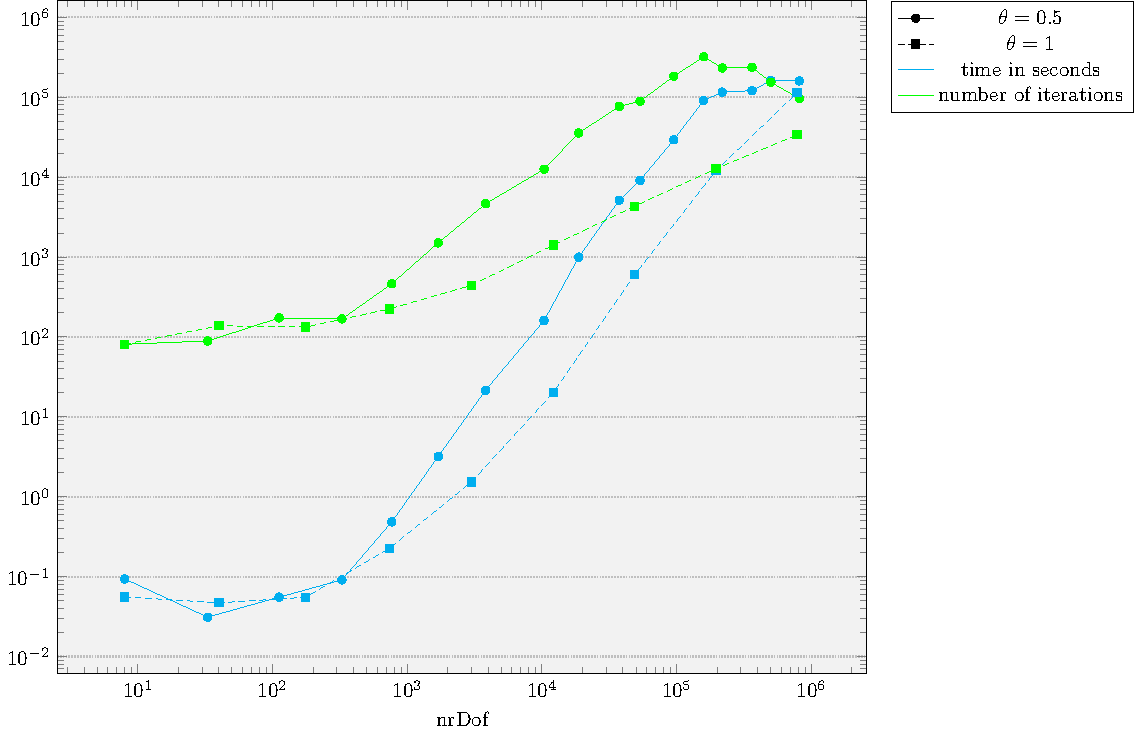
\includegraphics[width=14cm]{tikzPlots/middleSquare/misc.pdf}
  \caption{development of the number of iterations and the elapsed time for 
  each iteration}
\end{figure}

\begin{minipage}[t]{0.5\textwidth}
  \begin{figure}[H]
	  \centering
		\includegraphics[width=\textwidth]
      {tikzPlots/middleSquare/1e-4/adaptive/lvl16/solutionGrayscale.png}
    \caption{grayscale plot of last iterate for $\theta = 0.5$}
  \end{figure}
\end{minipage}
\begin{minipage}[t]{0.5\textwidth}
  \begin{figure}[H]
	  \centering
		\includegraphics[width=\linewidth]
      {tikzPlots/middleSquare/1e-4/uniform/lvl8/solutionGrayscale.png}
    \caption{grayscale plot of last iterate for $\theta = 1$}
  \end{figure}
\end{minipage}

\DTLloaddb{db}{
tikzPlots/middleSquare/1e-4/adaptive/lvl8/currentDataReduced.csv}
\DTLassign{db}{1}{\nrNodes=nrNodes, \nrDof=nrDof}

\begin{figure}[H]
	\centering
  \includegraphics[width=14cm]
  {tikzPlots/middleSquare/1e-4/adaptive/lvl8/triangulation.png}
  \caption{adaptive mesh for $\theta = 0.5$ with \nrNodes\ nodes and 
  \nrDof\ degrees of freedom}
\end{figure}

\DTLgdeletedb{db}

\end{document}
